\newgeometry{top=1cm, bottom=2cm}
\section{Determinante}
\begin{figure}[h!]
    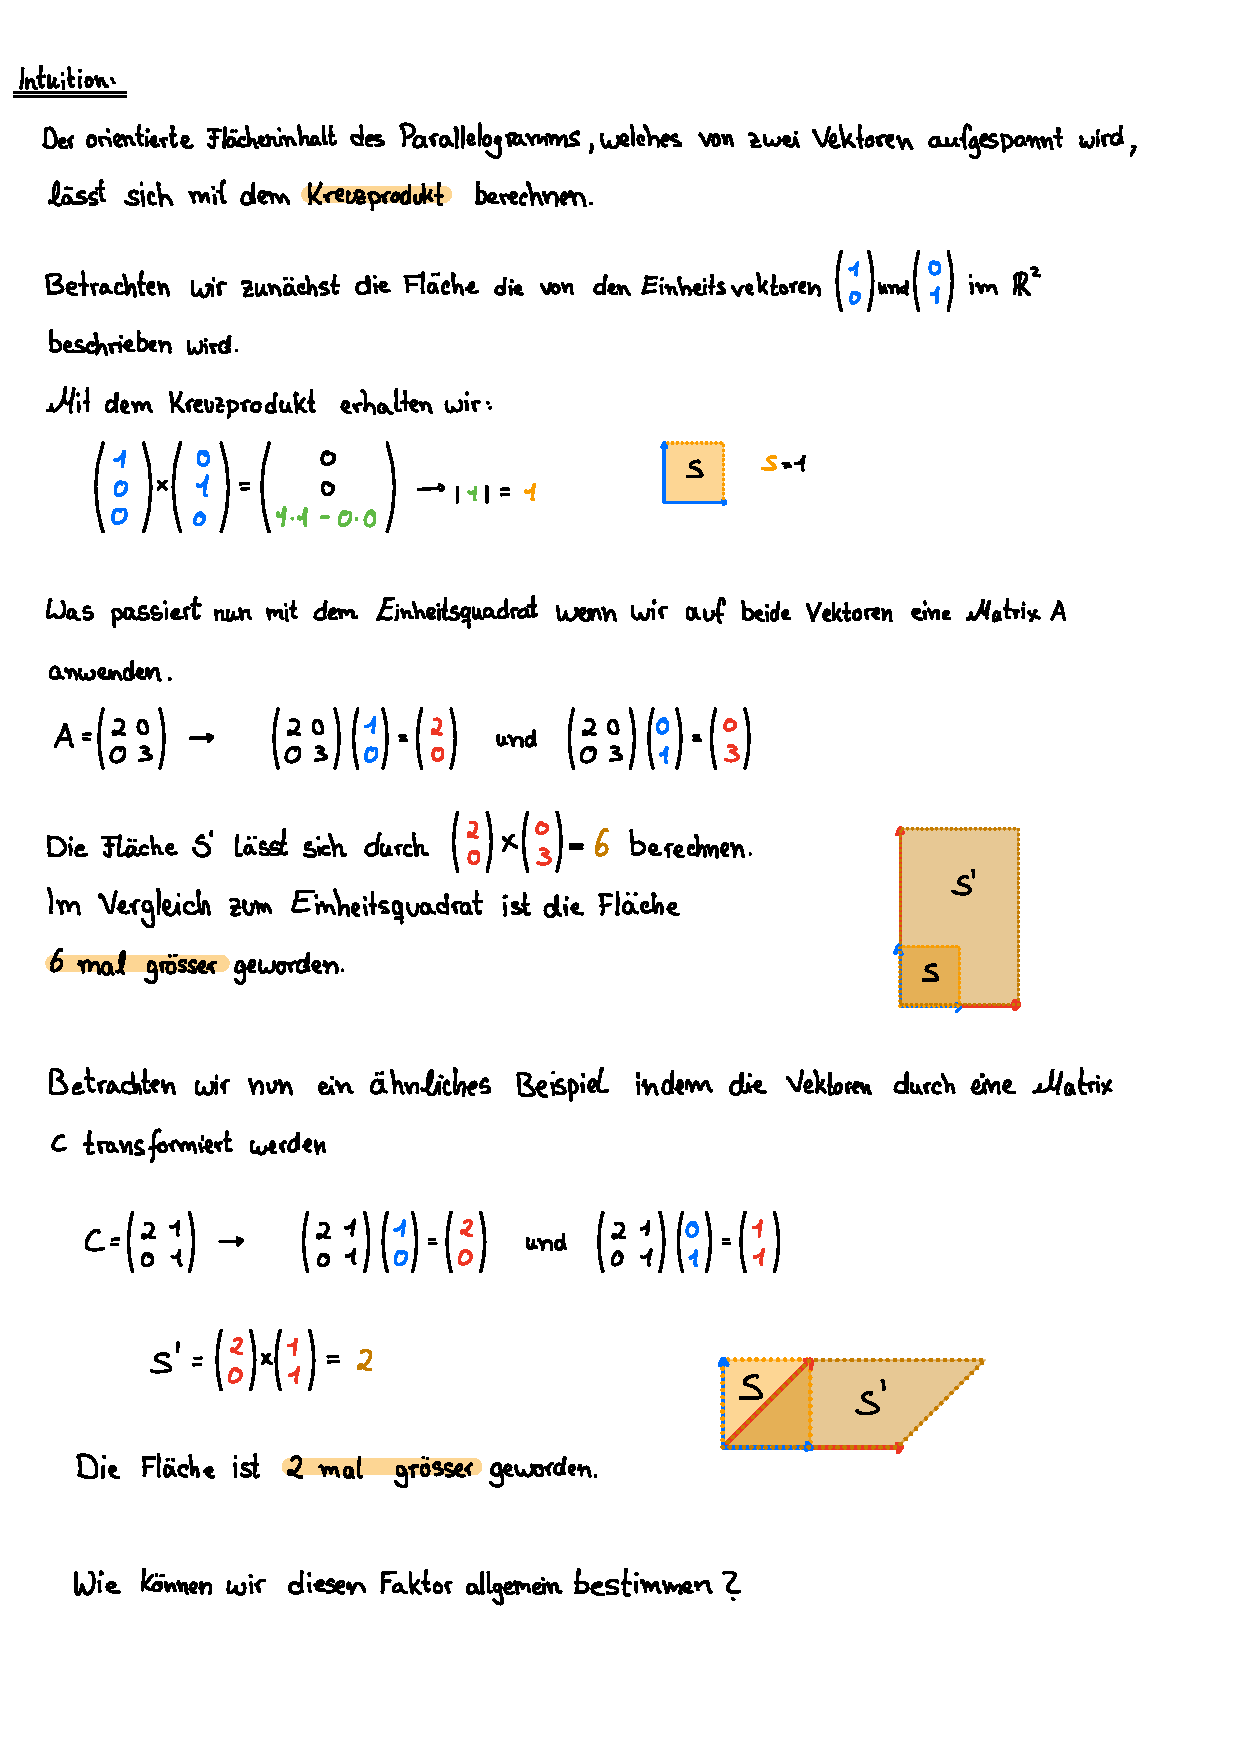
\includegraphics[page=1, scale=0.842]{pdf/03_Determinante.pdf}
\end{figure}
\newpage
\includepdf[pages={2-}, 
            pagecommand={\thispagestyle{plain}}, 
            scale=0.95]{pdf/03_Determinante.pdf}

\newgeometry{top=2.5cm, bottom=2cm}

\subsection{Beispielaufgaben} 

\vspace{1cm}

\subsubsection{} % Zardini S. 36

Sei
\begin{equation*}
    A = \begin{pmatrix}
    1 & 4 & 8 \\
    3 & 4 & 6 \\
    2 & 1 & 1
    \end{pmatrix}
\end{equation*}

Berechne det\((A^\top)\). 

\vspace{1\baselineskip}

\begin{solution}    

    \vspace{1\baselineskip}

    \leftskip=2em

    \begin{equation*}
        \begin{aligned}    
            A^\top = \begin{pmatrix}
            1 & 3 & 2 \\
            4 & 4 & 1 \\
            8 & 6 & 1 
            \end{pmatrix} \rightarrow \text{det}(A^\top) &= 4 + 24 + 48 - 64 - 6 - 12 \\
            &= -6 \\
            &= \text{det}(A) 
        \end{aligned}
    \end{equation*}

\end{solution}

\vspace{3cm}

\subsubsection{}

Sei 

\begin{equation*}
    A = \begin{pmatrix}
    1 & 2 \\
    3 & 4 \\
    \end{pmatrix}
\end{equation*}

Berechne det\((A^{-1})\).

\vspace{1\baselineskip}

\begin{solution}    

    \vspace{1\baselineskip}

    \leftskip=2em

    \begin{equation*}
        \begin{aligned}
            \text{det}(A^{-1}) &= \frac{1}{\text{det}(A)} \\[0.5em]
            & \quad \; \: \text{det}(A) = 4 -6 = -2 \\[0.5em]
            \text{det}(A^{-1}) &= - \frac{1}{2}
        \end{aligned}            
    \end{equation*}

\end{solution}

\newpage

\subsubsection{} %Zardini S. 42

Seien $a, b, c, d \in \mathbb{R}$ und

\begin{equation*}
    M = \begin{pmatrix}
    a & 0 & 0 & 0 & 0 & 0 \\
    1 & -2 & 0 & -1 & 0 & 0 \\
    2 & b & 0 & 3 & 0 & 0 \\
    0 & 7 & 1 & -2 & 0 & 0 \\
    -1 & 4 & 0 & 7 & -1 & c \\
    5 & 1 & d & 4 & 1 & 2 \\
    \end{pmatrix}.
\end{equation*}

\begin{enumerate}[label=\alph*)]
    \item Berechnen Sie det\((M)\)
    \item Für welche \( a, b, c, d \) ist \( M \) singulär?
\end{enumerate}

\vspace{1\baselineskip}

\begin{solution}    

    \vspace{1\baselineskip}

    \leftskip=2em

    \textbf{a)} Hier benutzten wir den Blocksatz

    \begin{equation*}
        \text{det} \begin{pmatrix}
            \textcolor{orange}{a} & \textcolor{orange}{0} & \textcolor{orange}{0} & \textcolor{orange}{0} & \textcolor{red}{0} & \textcolor{red}{0} \\
            \textcolor{orange}{1} & \textcolor{orange}{-2} & \textcolor{orange}{0} & \textcolor{orange}{-1} & \textcolor{red}{0} & \textcolor{red}{0} \\
            \textcolor{orange}{2} & \textcolor{orange}{b} & \textcolor{orange}{0} & \textcolor{orange}{3} & \textcolor{red}{0} & \textcolor{red}{0} \\
            \textcolor{orange}{0} & \textcolor{orange}{7} & \textcolor{orange}{1} & \textcolor{orange}{-2} & \textcolor{red}{0} & \textcolor{red}{0} \\
            \textcolor{RoyalBlue}{-1} & \textcolor{RoyalBlue}{4} & \textcolor{RoyalBlue}{0} & \textcolor{RoyalBlue}{7} & \textcolor{ForestGreen}{-1} & \textcolor{ForestGreen}{c} \\
            \textcolor{RoyalBlue}{5} & \textcolor{RoyalBlue}{1} & \textcolor{RoyalBlue}{d} & \textcolor{RoyalBlue}{4} & \textcolor{ForestGreen}{1} & \textcolor{ForestGreen}{2} 
            \end{pmatrix} = \text{det}(\textcolor{orange}{\blacksquare}) \cdot \text{det}(\textcolor{ForestGreen}{\blacksquare}),
    \end{equation*}

    und berechnen die Determinanten der Blöcke einzeln.

    \begin{equation*}
        \begin{aligned}
            \text{det}(\textcolor{orange}{\blacksquare}) &= \begin{vmatrix}
            a^{\textcolor{Gray}{+}} & 0 & \textcolor{Gray}{0} & 0 \\
            1^{\textcolor{Gray}{-}} & -2 & \textcolor{Gray}{0} & -1 \\
            2^{\textcolor{Gray}{+}} & b & \textcolor{Gray}{0} & 3 \\
            \textcolor{Gray}{0^-} & \textcolor{Gray}{7^+} & \textcolor{Gray}{1^-} & \textcolor{Gray}{-2} 
            \end{vmatrix} \stackrel{\mathrm{\text{3. Sp.}}}{=} - \begin{vmatrix}
                a & 0 & 0 \\
                1 & -2 & -1 \\
                2 & b & 3 
            \end{vmatrix} = - (-6a + ab) = 6a-ab \\[0.75em]
            \text{det}(\textcolor{ForestGreen}{\blacksquare}) &= \begin{vmatrix}
                -1 & c \\
                1 & 2
            \end{vmatrix} = -2 - c
        \end{aligned}
    \end{equation*}

    Schliesslich erhalten wir 

    \begin{equation*}
        \text{det}(M) = (6a - ab)(-2 - c) = a(b-6)(2+c)
    \end{equation*}

    \vspace{1\baselineskip}

    \textbf{b)} \(M\) ist singulär, wenn \(\text{det}(M) = 0\). 

    \begin{equation*}
        a(b-6)(2+c) = 0
    \end{equation*}

    \( M \) ist singulär, wenn

    \begin{equation*}
        a = 0 \ \text{oder} \ b = 6 \ \text{oder} \ c = -2.
    \end{equation*}

\end{solution}

\newpage

\subsubsection{}%Zardini S. 51

Seien \( a, b, c, d \in \mathbb{R} \) und

\begin{equation*}
    A = \begin{pmatrix}
    a & b & c & d \\
    -3a & 2b & 3c & 2d \\
    a & b & -c & d \\
    -2a & -2b & -2c & d \\
    \end{pmatrix}.
\end{equation*}

Berechnen Sie die Determinante von \( A \). 

\vspace{1\baselineskip}

\begin{solution}    

    \vspace{1\baselineskip}

    \leftskip=2em

    Durch das Addieren eines Vielfachen einer Zeile zu einer anderen ändert die Determinante nicht. Das können wir ausnutzten und anschliessend nach der 3. Zeile entwickeln.

    \begin{equation*}
        \begin{gmatrix}[v]
            a & b & c & d \\
            -3a & 2b & 3c & 2d \\
            a & b & -c & d \\
            -2a & -2b & -2c & d 
                \rowops
                    \add[-1]{0}{2}
        \end{gmatrix} = \begin{vmatrix}
            a^{\textcolor{Gray}{+}} & b^{\textcolor{Gray}{-}} & \textcolor{Gray}{c^+} & d \\
            -3a & 2b & \textcolor{Gray}{3c^-} & 2d \\
            \textcolor{Gray}{0} & \textcolor{Gray}{0} & \textcolor{Gray}{-2c^+} & \textcolor{Gray}{0} \\
            -2a & -2b & \textcolor{Gray}{-2c} & d
        \end{vmatrix} = -2c \begin{vmatrix}
            a & b & d \\
            -3a & 2b & 2d \\
            -2a & -2b & d
        \end{vmatrix}
    \end{equation*}

    Schliesslich benutzten wir die Regel von Sarrus, um die 3\(\times\)3 Determinante zu berechnen. 

    \begin{equation*}
        \begin{aligned}
            \text{det}(A) &= -2c(2abd - 4abd + 6abd + 4abd + 4abd + 3abd) \\[0.5em]
            &= -2c(15abd) \\[0.5em]
            &= -30abcd
        \end{aligned}
    \end{equation*}


\end{solution}

\newpage

\subsubsection{}

Seien \( a, b, c, d \in \mathbb{R} \) und

\begin{equation*}
    A = \begin{pmatrix}
    a & b & c & d & b & b & d \\
    b & c & d & d & b & d & a \\
    c & d & b & c & d & c & c \\
    d & b & c & d & b & b & c \\
    b & d & c & b & d & b & b \\
    b & c & d & d & b & d & a \\
    d & a & c & d & a & b & c 
    \end{pmatrix}.
\end{equation*}

Berechnen Sie die Determinante von \( A \).

\vspace{1\baselineskip}

\begin{solution}    

    \vspace{1\baselineskip}

    \leftskip=2em

    \begin{equation*}
    A = \begin{pmatrix}
    a & b & c & d & b & b & d \\
    \textcolor{orange}{b} & \textcolor{orange}{c} & \textcolor{orange}{d} & \textcolor{orange}{d} & \textcolor{orange}{b} & \textcolor{orange}{d} & \textcolor{orange}{a} \\
    c & d & b & c & d & c & c \\
    d & b & c & d & b & b & c \\
    b & d & c & b & d & b & b \\
    \textcolor{orange}{b} & \textcolor{orange}{c} & \textcolor{orange}{d} & \textcolor{orange}{d} & \textcolor{orange}{b} & \textcolor{orange}{d} & \textcolor{orange}{a} \\
    d & a & c & d & a & b & c 
    \end{pmatrix} \rightarrow II = VI, \ \text{also det}(A) = 0.
\end{equation*}    

\end{solution}
